\begin{figure}[htb]
    \centering
    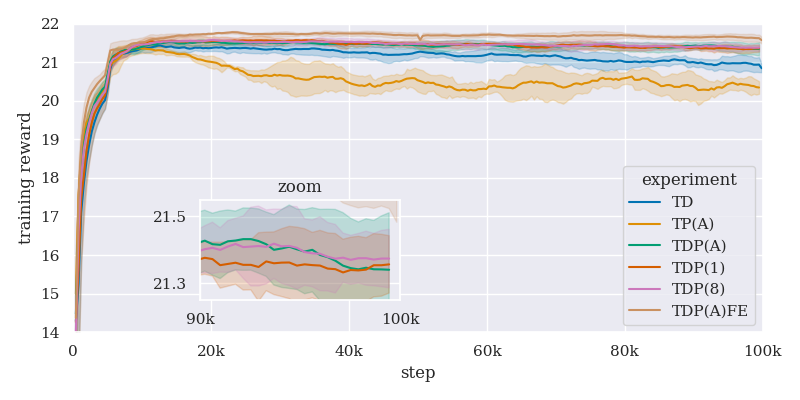
\includegraphics[width=0.75\linewidth]{Figures/rewards_zoom.png}
    \caption{The training reward during the training process. The shaded area represents the standard deviation over the five repetitions. The lines of the different pressure sensor configurations are included in a zoomed in window, since they overlap heavily.}
    \label{fig:reward_training}
\end{figure}



The episodic returns over the course of all  training runs are depicted in Fig. \ref{fig:reward_training}.
The plotted results reveal, that all observation types are beneficial for the agent to reach a higher reward.
However, while adding pressure values to the observation in general results in a clearly visible improvement, the amount of sensors matters relatively little.
The reward curves are nearly indistinguishable from one another. Furthermore
the standard deviation is small in comparison between the experiments \textit{TD} and \textit{TP(A)}, so the curves are similar regardless of the random sensor locations.

% \begin{table}
%     \centering
%     \begin{tabular}{l|c|c|c}
%          Experiment & Pressure & Price & Smoothness\\
%          \hline
%          TD & $0.999 (.018)$ & $0.607 (.159)$ & $0.940 (.055)$\\
%          TP(A) & $0.999 (.009)$ & $0.588 (.164)$ & $0.951 (.043)$\\
%          TDP(A) & $1.000 (.011)$ & $0.606 (.172)$ & $0.947 (.060)$\\
%          TDP(1) & $0.999 (.012)$ & $0.602 (.173)$ & $0.932 (.073)$\\
%          TDP(8) & $\mathbf{1.000 (.005)}$ & $0.596 (.153)$ & $\mathbf{0.961 (.049)}$ \\
%          TDP(A)FE & $\mathbf{1.000 (.005)}$ & $\mathbf{0.652 (.261)}$ & $0.667 (.214)$\\
%     \end{tabular}
%     \caption{This table lists the mean partial rewards the agents reached after training per time step. The standard deviation is given in parentheses.}

%     \label{tab:rewards}
% \end{table}

\begin{wraptable}[12]{r}{65mm}
    \begin{tabular}{l|c|c}
         Experiment & Pressure & Price \\
         \hline
         TD & $0.999 (.018)$ & $0.607 (.159)$\\
         TP(A) & $0.999 (.009)$ & $0.588 (.164)$\\
         TDP(A) & $1.000 (.011)$ & $0.606 (.172)$\\
         TDP(1) & $0.999 (.012)$ & $0.602 (.173)$\\
         TDP(8) & $\mathbf{1.000 (.005)}$ & $0.596 (.153)$\\
         TDP(A)FE & $\mathbf{1.000 (.005)}$ & $\mathbf{0.652 (.261)}$\\
    \end{tabular}
    \caption{This table lists the mean partial rewards the agents reached after training per time step. The standard deviation is given in parentheses.}
    \label{tab:rewards}
\end{wraptable}

For a more detailed look into the performance of the fully trained agents we refer to Tab. \ref{tab:rewards}.
The table splits the reward into its components of keeping all nodes within pressure bounds and optimizing the operation costs of the pumps.
All agents have managed to find a policy to stay within the pressure bounds at all nodes with only small deviations.
The price objective gains another noticable boost from the added flow and energy consumption information.
However, while inspecting the policy over the course of one day, we found that
the agent gained that boost by learning to switch the pump on and off every
other hour. Using an additional reward term to discourage this behaviour is
part of our ongoing research.
%Hence, we added a third column, which evaluates the smoothness of the learned policies, ensuring no overly large changes within the last three steps.
%All other agents do not follow a disruptive pattern like that.


%The similar performances of different pressure sensors show that sparse sensor placements are sufficient to factor in pressure for pump schedule optimization.
%It remains an open question how this scales to larger networks, where pressure will be more varied over nodes and sensor locations may become more important.
%While we started experimenting with larger networks, some of the problems we encountered were uncertainty of whether all pressure bounds could be fulfilled, instable hydraulic states during exploration and runtime.
